\chapter{\label{Packaging}Packaging}
This chapter describes the way how modules (packages) are transfered between Kistl installations.

\section{\label{Packaging_Content_of_a_package}Content of a package}

A package contains schema information, meta data, object instances and code. See \ref{content_of_package} for details. 
A package can contain one or more modules. A package is a zip file that contains one or more XML files containing meta information and/or data and binary files like icons or assemblies.

\begin{figure}[ht]
	\begin{center}
		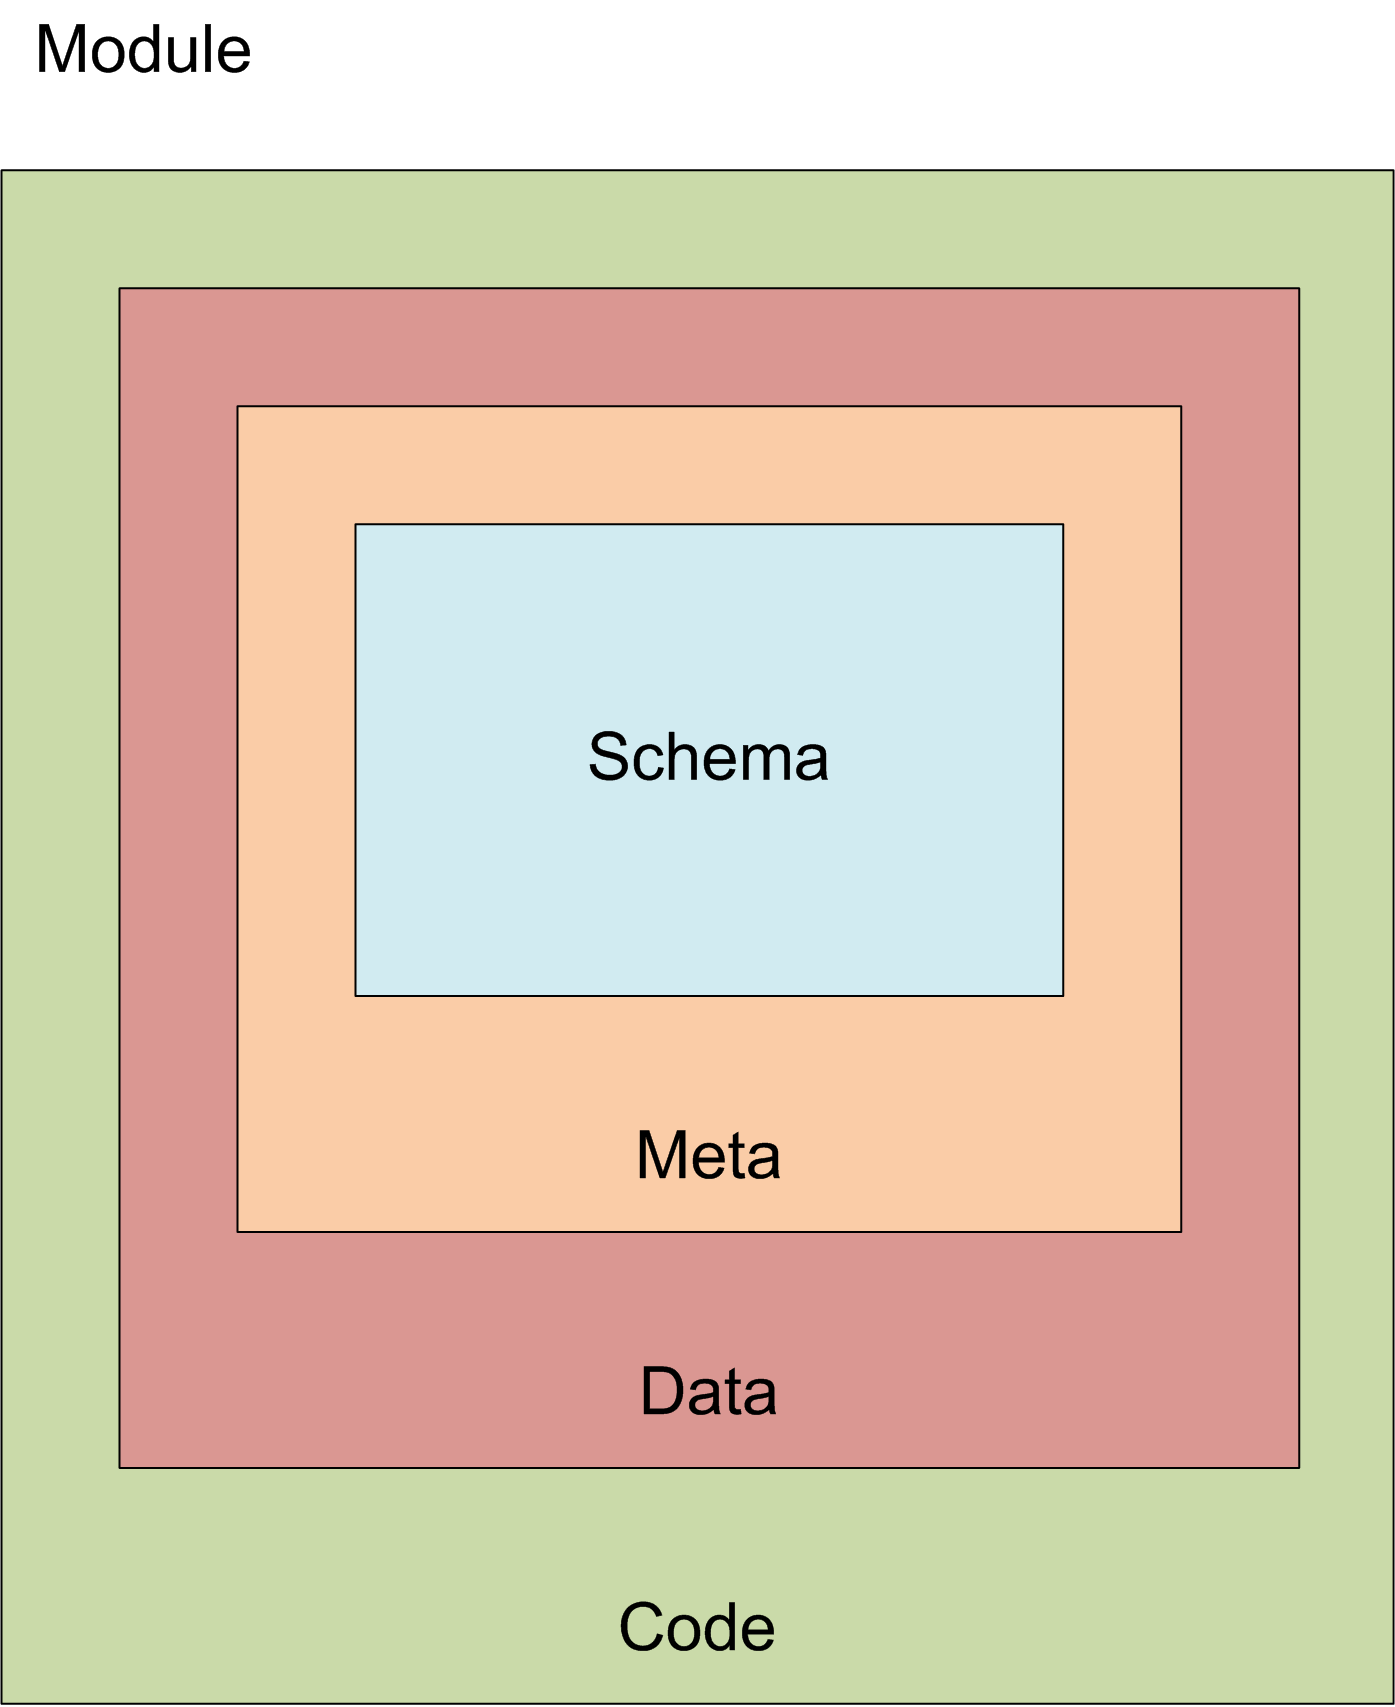
\includegraphics[width=0.6\textwidth]{images/content_of_package.png}
		\caption{Content of a package}
		\label{content_of_package}
	\end{center}
\end{figure}

\subsection{\label{Packaging_Schema}Schema}

Schema contains all information needed by the SchemaManager \ref{} to create or update the database. Schema objects are:

\begin{descriptionBorder}
	\item[DataType] { All object classes and structs except enumerations and interfaces. \emph{To be implemented!} }
	\item[Property] { All properties }
	\item[Relation] { All relations }
	\item[RelationEnd] { All relation ends }
	\item[DefaultPropertyValue] { All known default property values (IntDefaultValue, \ldots) }
	\item[Constraint] { All known constraints (NotNullable, \ldots) }
\end{descriptionBorder}

\par
Schema is a subset of meta data. See \ref{Packaging_Meta}. Currently there is no way to extract schema information without meta information.


\subsection{\label{Packaging_Meta}Meta}

Meta data contains all information needed to describe a Module. That are \emph{ObjectClasses}, \emph{TypeRefs}, \emph{Module} informations, \emph{icons}, \emph{ViewDescriptors} and so on. 
Meta data is a superset of schema data \ref{Packaging_Schema}. These objects are:

\begin{descriptionBorder}
	\item[Module] { The module object }
	\item[ObjectClass\_implements\_Interface\_RelationEntry] { All object class interface relations }
	\item[Method] { All Methods }
	\item[BaseParameter] { All parameter of a method }
	\item[MethodInvocation] { All method invocations }
	\item[PropertyInvocation] { All property invocations (getter/setter) }
	\item[Assembly] { All Assemblies (meta information only, not code) }
	\item[TypeRef] { All type references }
	\item[TypeRef\_hasGenericArguments\_TypeRef\_RelationEntry] { All generic arguments of type references. }
	\item[Icon] { All Icons (descriptor only, no binary data) }
	\item[PresentableModelDescriptor] { All presentable model descriptors }
	\item[ViewDescriptor] { All view descriptors }
	\item[DAVID: ] { please add more GUI objects here. And please do it also in \emph{PackagingHelper.GetMetaObjects(\ldots)} }
\end{descriptionBorder}

Additionally all unknown DefaultPropertyValues and Constraints belongs to meta data.
Meta data can be extracted with the publish command \ref{Packaging_Publish}.

\subsection{\label{Packaging_Data}Data}

A package can also contain additional data. Only object classes that implements \emph{IExportable} will be exported. 
N:M relations between object classes that implements \emph{IExportable} are also exported. 
Currently all objects of a specific module are exported.
Data can be extracted with the export command \ref{Packaging_Export}.

\subsection{\label{Packaging_Code}Code}

Finally a package consists of code in form of assemblies. These assemblies are referenced by \emph{Assembly} objects.

\section{\label{Packaging_Processes}Processes}

\subsection{\label{Packaging_Export}Export}

Exporting is the process of saving objects in XML files. Only object classes that implements \emph{IExportable} will be exported. 
N:M relations between object classes that implements \emph{IExportable} are also exported. 
Currently all objects of a specific module are exported.

Command line for exporting objects:
\begin{CS}
Kistl.Server <configfile.xml> -export <destfile.xml> <namespace> [<namespace> ...]
\end{CS}

The namespace is used to identify a module. \emph{TODO: Work in progress. This is not the best solution!}
\par

This example will export all objects of the project management module:
\begin{CS}
Kistl.Server -export Export.xml Kistl.App.Projekte
\end{CS}

This example will export \emph{all} meta data of \emph{all} modules:
\begin{CS}
Kistl.Server -export Export.xml Kistl.App.Base Kistl.App.GUI
\end{CS}

This example will export the whole database:
\begin{CS}
Kistl.Server -export Export.xml *
\end{CS}

\subsection{\label{Packaging_Import}Import}

Importing is the inverse process of exporting \ref{Packaging_Export}. Objects are imported by the following rules:

\begin{enumerate}
 \item If an imported object already exists in the target database then the object will be overridden
 \item New objects are added
 \item No object is deleted if it's not contained in the package
\end{enumerate}

Command line for importing objects:
\begin{CS}
Kistl.Server <configfile.xml> -import <sourcefile.xml>
\end{CS}

\subsection{\label{Packaging_Publish}Publish}

Publishing is a special case of exporting \ref{Packaging_Export}. Only meta data \ref{Packaging_Meta} of a given module will be exported. 
Additionally only properties of the Kistl.App.Base and Kistl.App.GUI module are published.

Command line for publishing modules:
\begin{CS}
Kistl.Server <configfile.xml> -publish <destfile.xml> <namespace> [<namespace> ...]
\end{CS}

The namespace is used to identify a module. \emph{TODO: Work in progress. This is not the best solution!}
\par

This example will publish the project management module:
\begin{CS}
Kistl.Server -publish Meta.xml Kistl.App.Projekte
\end{CS}

This example will publish all modules:
\begin{CS}
Kistl.Server -publish Meta.xml *
\end{CS}


\subsection{\label{Packaging_Deploy}Deploy}

Deployment is the inverse process of publishing \ref{Packaging_Publish}. It also has different rules (see importing \ref{Packaging_Import}).
These Rules are:

\begin{enumerate}
 \item If an imported object already exists in the target database then the object will be overridden
 \item Only properties of the the Kistl.App.Base and Kistl.App.GUI module are overriden.
 \item New objects are added
 \item Any object that is not contained in the packed will be deleted
\end{enumerate}

Command line for importing objects:
\begin{CS}
Kistl.Server <configfile.xml> -deploy <sourcefile.xml>
\end{CS}

The database schema is not updated. Also no code is generated. This has to be done in an extra step.